\documentclass{article}
\usepackage[utf8]{inputenc}

\title{\HUGE TFIM Model}
\author{Rok Mlinar Vahtar}
\date{August 2023}
\usepackage[slovene]{babel}
\usepackage[none]{hyphenat}
\usepackage{subcaption}
\usepackage{mwe}
\usepackage{graphicx}
\usepackage[margin=1in]{geometry}
\usepackage{svg}
\usepackage{amsmath}
\graphicspath{ {./SkNiKr/} }

\begin{document}

\maketitle

\section{Uvod}
\textless \hspace{1pt} tu vstavi fenomenalno napisan uvod \textgreater

\section{Standardni TFIM model}
Hamiltonian za standardni Isingov model z tranzverzalnim poljem se glasi
\begin{equation}
    \hat{H} = \sum_{< i,j >} -J \hat{\sigma_i^z} \hat{\sigma_j^z} - h\sum_i \hat{\sigma_i^x} - J_T \sum_i
\end{equation}
in ga za dimenzije $N < 10$ lahko rešimo z direktno diagonalizacijo v doglednem času. Vse naslednje metode, predstavljene v tem poglavju se nahajajo v datoteki TFIM\_QuSpin.py . Dobra mera za stanje sistema, ki nas bo tu zanimala, je magnetizacija, ki jo definiramo kot:
\begin{equation}
    M = \frac{1}{N}\sum_{i=0}^N \sigma_i^z
\end{equation}\\
Če fiksiramo J = 1 in variiramo h, ter vsakič izračunamo magnetizacijo, dobimo naslednji graf, ki kaže fazni prehod pri $h \approx J$. To opravlja funkcija main().

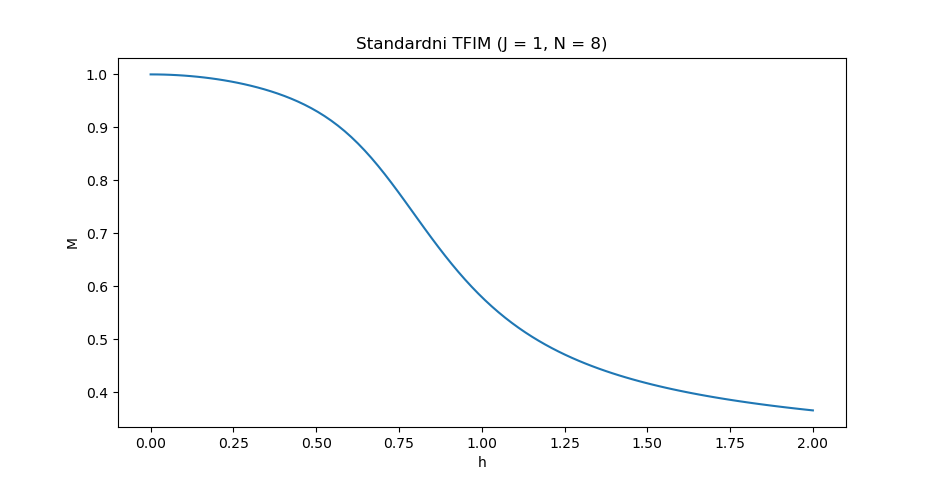
\includegraphics[width = \linewidth]{STFIM1.png}

\newpage
\noindent Če variiramo oba J in h lahko narišemo 3D in contour grafa, na katerih opazimo pričakovane lastnosti, kot so simetrija čez ravnino h = 0 in pa feromagnetno in antiferomagnetno obnašanje za $J > 0$ in $J < 0$.\\\\

\begin{tabular}{c c}
     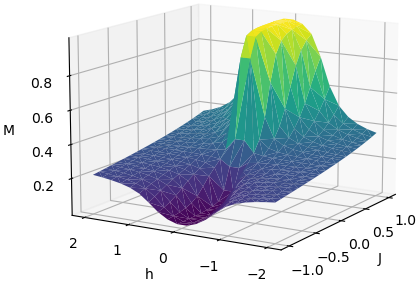
\includegraphics[width = .5 \linewidth]{STFIM2.png}
     &  
     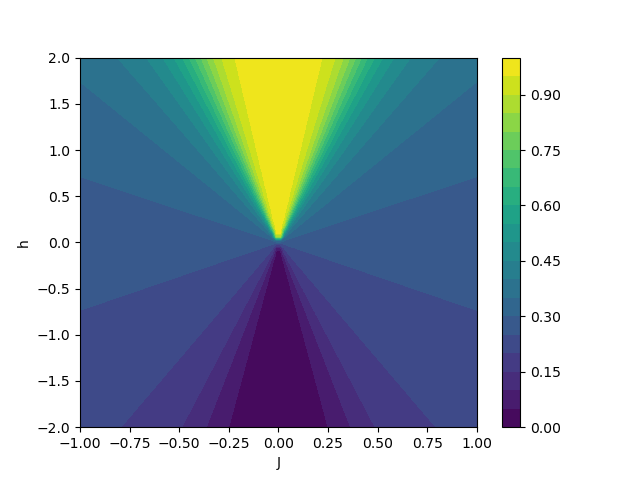
\includegraphics[width = .5 \linewidth]{STFIM3.png}\\
\end{tabular}
Grafa narisana preko plot3d() in plot\_contour().


\section{Sklopljeni verigi}
Hamiltonian se glasi
\begin{equation}
    \hat{H} = \sum_{< i,j >} -J \hat{\sigma_{1i}^z} \hat{\sigma_{1j}^z} + \sum_{< i,j >} -J \hat{\sigma_{2i}^z} \hat{\sigma_{2j}^z} - h\sum_i \hat{\sigma_{1i}^x}- h\sum_i \hat{\sigma_{2i}^x} - J_T \sum_i \hat{\sigma_{1j}^z} \hat{\sigma_{2i}^z}
\end{equation}
in ga za dimenzije $N < 10$ lahko rešimo z direktno diagonalizacijo v doglednem času. Vse naslednje metode, predstavljene v tem poglavju se nahajajo v datoteki TFIM\_QuSpin\_2.py . Dobra mera za stanje sistema, ki nas bo tu zanimala, je magnetizacija, ki jo definiramo kot:

\noindent Če variiramo oba $h$ ter $J_T$ pri fiksnem $J = 1$ lahko narišemo 3D in contour grafa\\\\

\begin{tabular}{c c}
     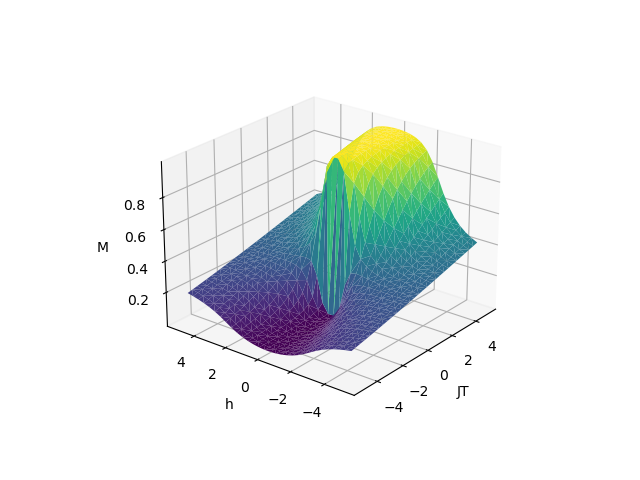
\includegraphics[width = .5 \linewidth]{2TFIM1.png}
     &  
     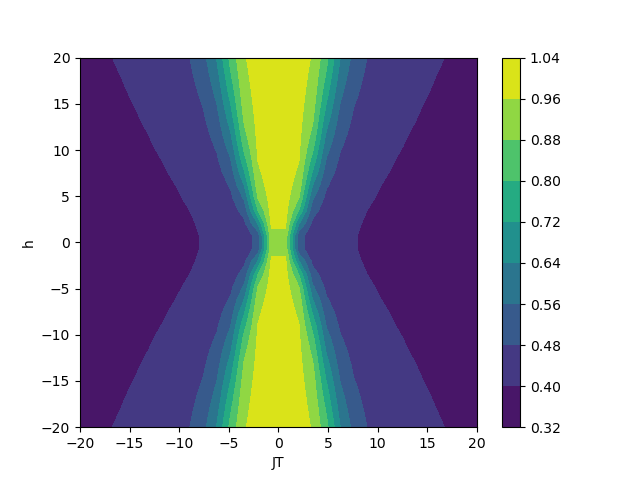
\includegraphics[width = .5 \linewidth]{2TFIM2.png}\\
\end{tabular}
Grafa narisana preko plot3d() in plot\_contour().


\end{document}
